\chapter{Introduction}
The goal of this text is to teach mathematical and computer science concepts through a series of stories
that are designed for students in grades 7-10.

The storyline is similar to the Vikramaditya stories, also called the Vetal tales, in Indian folklore. These stories are believed to have taken place in the 11th century BCE.\footnote{\url{https://en.wikipedia.org/wiki/List_of_Vetala_Tales}}
Collectively, there are 21 stories, one taking place each night. Each story begins with a series of questions, and the protagonist has to successfully answer those questions to set himself free. 


Our stories start on October 31st, Halloween, and continue nightly for 25 subsequent nights. They take place in a hamlet called Royt, a small college town somewhere in Upstate New York. Royt was a prosperous town a hundred years ago, but these days the town has many dilapidated buildings and a rather imposing cemetery. Ajur and his parents live in this hamlet. Ajur has a pet dog named Jura who accompanies Ajur wherever he goes.  In the cemetery lives Rishnak, a ghost who was a tyrant but now has good intentions.

\section{Characters and setting}

\textbf {Ajur} - A young boy who is interested in mathematics but easily gets bored.\\
\noindent
\textbf {Jura} - Ajur's pet dog.\\
\noindent
\textbf{Kinaja} - An angel who helps Ajur overcome the challenges posed by Rishnak.\\
\noindent
\textbf{Rishnak} - A ghost with a mathematical bent from whom Ajur wants to escape by solving various mathematical challenges.\\
\noindent
\textbf{Royt} - The hamlet in which the entire story takes place, home of the most famous cemetery in the country.

\begin{newpage}
\end{newpage}
\section{Notation}
\textbf{Graphs}, also known as networks, occur naturally in many different applications. They are abstractions of a relation between any two objects: a binary relation. Objects can for example be people, cities, countries, or web-pages. These objects are represented by \textbf{vertices}, usually drawn as dots 
or circles on a page. Relations may exist between any two different objects. These relations are represented as lines connecting the two vertices, called \textbf{edges}.

We will illustrate with three examples. In example one [Figure \ref{1g1}], there are four vertices representing objects, the numbers 0, 1, 2 and 3. There are six relations (or six edges): these relations are \{0,1\}, \{0,2\}, \{0,3\}, \{1,2\}, \{1,3\} and \{2,3\}. These relations are symmetric --- that is if there is a relation between vertex 0 and vertex 1, then there is also a relation between vertex 1 and vertex 0. Such graphs are called \textbf{undirected} graphs.
\begin{figure}
\begin{center}
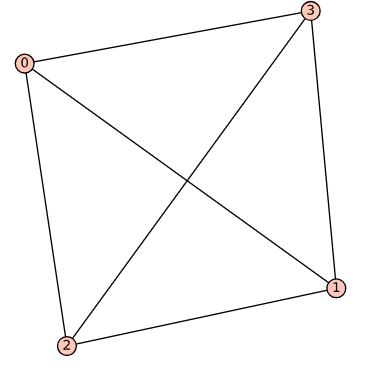
\includegraphics[width=0.6\textwidth]{example.JPG}
\caption{A graph with 4 vertices and 6 edges}\label{1g1}
\end{center}
\end{figure}
\begin{newpage}
\end{newpage}

In our next example [Figure \ref{1g2}], we have five vertices, representing five persons, Bob, William, James, Chris and Ajur. The edges in the graph represent friendship. Chris is friends with William, James and Ajur. Bob is friends with William and James. This is depicted as a graph in Figure 1.2. It has 5 vertices and 5 edges.
\begin{figure}
\begin{center}
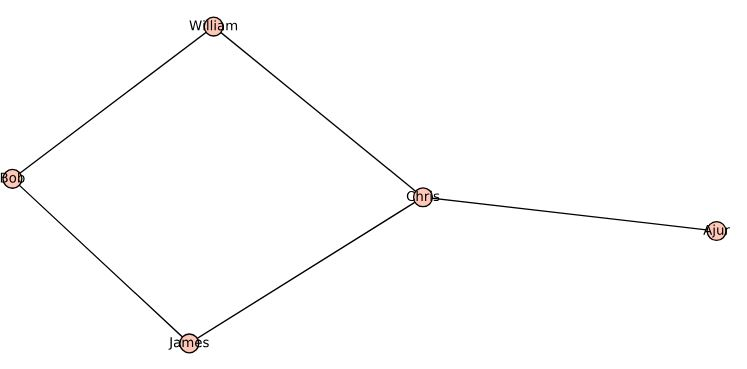
\includegraphics[width=0.9\textwidth]{example2.JPG}
\caption{A friendship graph with 5 vertices and 5 edges}\label{1g2}
\end{center}
\end{figure}
\begin{newpage}
\end{newpage}
In our third example [Figure 1.3], we have seven Northeastern states in the United States, namely NY (New York), CT (Connecticut), VT (Vermont), ME (Maine), MA (Massachusetts) RI (Rhode Island) and NH (New Hampshire). The relationship represented is sharing a border with another state. NY borders CT, VT, and MA. CT additionally borders RI and MA. VT borders MA and NH. ME borders NH. MA borders RI and NH. This is depicted in Figure \ref{1g3}. It has 7 vertices and 10 edges.

\begin{figure}
\begin{center}
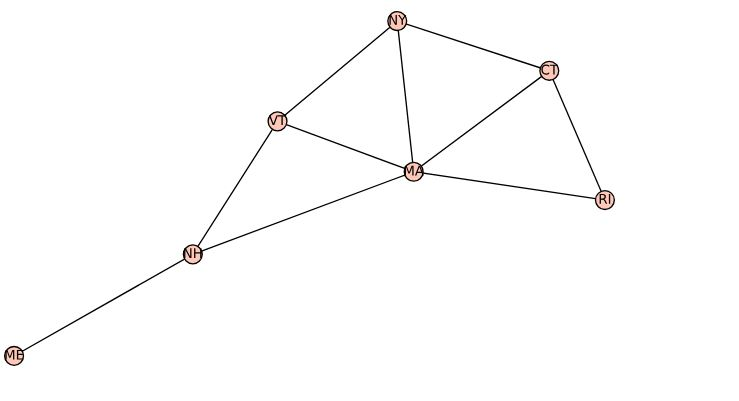
\includegraphics[width=0.9\textwidth]{example3.JPG}
\caption{A graph representing the northeastern United States, with 7 vertices and 10 edges}\label{1g3}
\end{center}
\end{figure}
\begin{newpage}
\end{newpage}

If there is an edge between two vertices (like NY and VT in Figure 1.3), we say that these two vertices are \textbf{adjacent}. For instance, NY is adjacent to VT and VT is adjacent to NY.

%\chapter{Introduction}
   

\chapter{Trip to the Cemetery}
It was a Halloween, a cold and dreary evening. Ajur was interested in visiting the famous cemetery in Royt as any teenager with an adventurous spirit would be. His pet dog Jura, a Labrador, was eager to follow him. As Ajur was examining the headstones and tombs, he lost track of time and it was getting dark. He grew tired and he and Jura sat under a tree and they fell asleep. Suddenly they were awakened by a loud noise. The noise was from Rishnak, a ghost who lived in the cemetery. Rishnak had died a few years ago; he used to teach mathematics and graph theory for talented high school students in the area. When Rishnak spotted Ajur in that cemetery, he thought to himself, ``here is an unusual teenager." Perhaps he could test whether this youngster  was proficient in mathematics. If he was indeed proficient, Rishnak could reward him with his magical powers. When Rishnak appeared in front of Ajur, Jura started barking.  

Rishnak was afraid he would intimidate Ajur by being brusque. Jura was barking with loudly. So Rishnak started talking in a soft voice. He gently asked what grade Ajur was in. Ajur replied that he was in middle school and studying in 8th grade. Rishank proceeded to ask the boy what subjects he liked most in school. Ajur proudly added that he was very good in mathematics. Rishnak smiled to himself. He told the boy that he had been cursed to live as ghost and his curse would be lifted if he could reward some youngsters who could answer all his questions. Ajur was intrigued by Rishnak's offer and he jumped at the possibility of rewards, and the opportunity to help lift the curse on a Rishnak, a ghost and tell his friends about his adventure.